\section{Multilagen-PVD}
\label{multilayer}

Der PVD-Modus von Parsivald ist durch seine zyklische Arbeitsweise auch für Multilagensysteme geeignet, wie in diesem Abschnitt am Beispiel von Cu/Ni-Multilagen untersucht wird.

\subsection{Vorbetrachtung}
Die Wahl fiel auf Kupfer-Nickel-Systeme aufgrund der ähnlichen Atom- und Gittereigenschaften sowie die Verfügbarkeit eines kompatiblen \todo{cite lammps?}Potentiales.
Diese Systeme können per \todo{cite}Elektro\-deposition oder durch \todo{cite}Sputtern hergestellt werden, wobei üblicherweise Lagendicken von \todo{cite!}\SI{5}{\angstrom} bis \todo{cite. angstrom oder nm?}\SI{200}{\angstrom} produziert werden.
\todo{wirklich?}Durch Beschränkungen in der verfügbaren Rechenzeit beschränken sich die vorgestellten Simulationen auf Lagendicken unterhalb von \SI{10}{\angstrom}, allerdings sind größere Systeme technisch möglich.

An Multilagensystemen lassen sich strukturell neben den Dicken der einzelnen Lagen die Rauheiten aufeinanderfolgender Schichten besonders gut untersuchen.
Man betrachtet die Korrelation zwischen den einzelnen Schichten sowie den Verlauf der Rauheit bei späteren Schichten.
Für das Cu/Ni-System werden \todo{Aus welchem Hut wurde das gezaubert?}partiell korrelierte, kumulative Rauheiten erwartet, wobei Untersuchungen an den Gold- und Kupfer-Strukturen der letzten Kapitel eine systematische Überschätzung des Verlaufs der Rauheiten vermuten lassen\todo{Hut?}.

\subsection{Ergebnisse}

Die in Abbildung \ref{fig:multilayerresults} vorgestellten Ergebnisse zeigen erfolgreiches Multilagenwachstum per PVD-Modus mit Diffusion einzelner Atome in benachbarte Lagen.
Die Atome der verschiedenen Lagen setzen das fcc-Kristallgitter der vorherigen Lage fort, was durch die Ähnlichkeit der fcc-Gitterkonstanten zu erklären ist (\SI{3.52}{\angstrom} für Nickel, \SI{3.61}{\angstrom} für Kupfer, entspricht \SI{2.5}{\percent} Abweichung).
Bei größeren Systemen sind durch Verspannungen im Material Gitterversetzungen und -fehlstellen zu erwarten, die allerdings durch \todo{Wort}Finite-Size-Effekte unterdrückt sein können.

\begin{figure}[hp]
  \captionsetup[subfigure]{singlelinecheck=false}
  \def\subfigwidth{7cm}
  %% \begin{subfigure}[t]{\subfigwidth}
  %%   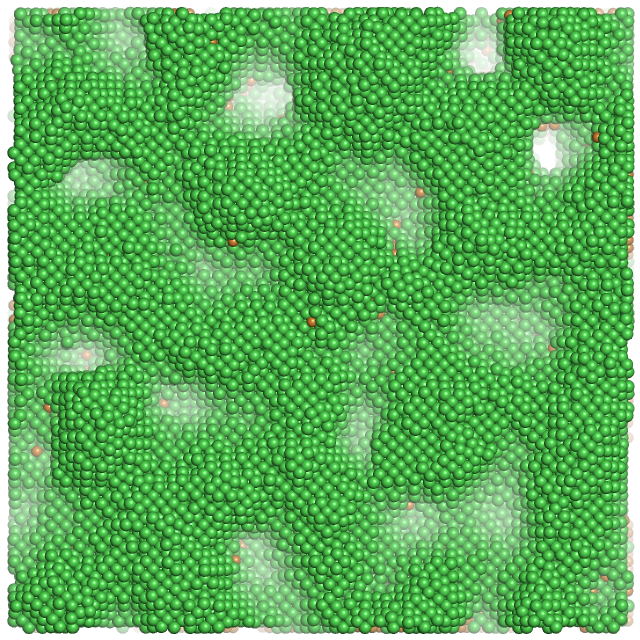
\includegraphics[width=\textwidth]{CuNi_surface8}
  %%   \subcaption{Top-Ansicht einer CuNi-Multi\-lagen\-ober\-fläche nach je 4 Lagen (insgesamt \SI{60}{\angstrom})}
  %% \end{subfigure}
  %% \hfill
  \begin{subfigure}[t]{\subfigwidth}
    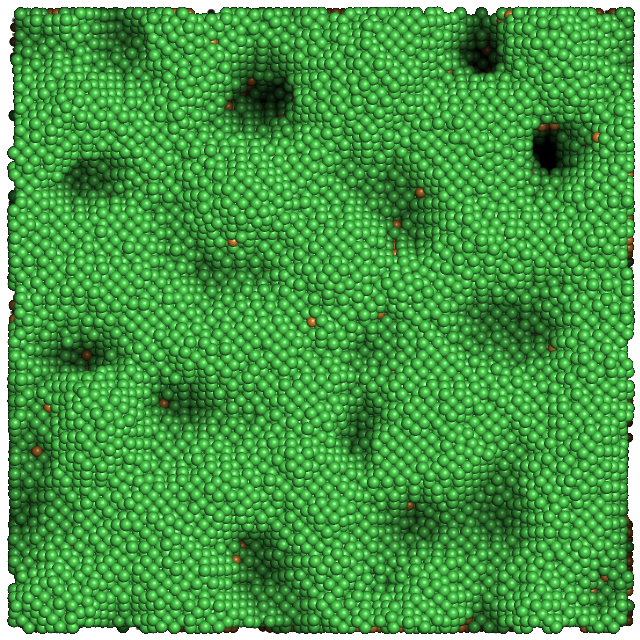
\includegraphics[width=\textwidth]{CuNi_surface8_noalpha}
    \subcaption{Top-Ansicht einer CuNi-Multi\-lagen\-ober\-fläche nach je 4 Lagen (insgesamt \SI{60}{\angstrom})}
  \end{subfigure}
  \hfill
  \begin{subfigure}[t]{\subfigwidth}
    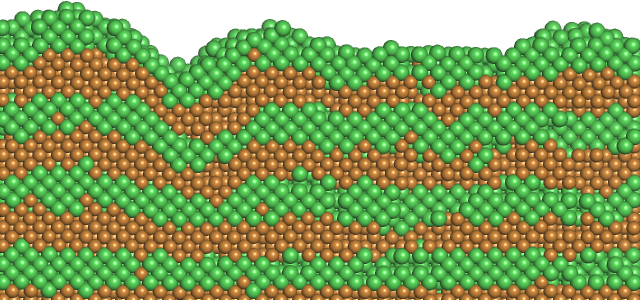
\includegraphics[width=\textwidth]{CuNi_profile8}
    \subcaption{Profil eines CuNi-Multi\-lagen\-systemes nach je 4 Lagen (insgesamt \SI{60}{\angstrom})}
  \end{subfigure}
  \caption[Ergebnisse bei Kupfer-Nickel-Multilagen-PVD]{Ergebnisse bei Kupfer-Nickel-Multilagen-PVD}
  \label{fig:multilayerresults}
\end{figure}

\todo[inline]{update with the results of 93\_*/23..28}
